%%%%%%%%%%%%%%%%%%%%%%%%%%%%%%%%%%%%%%%%%%%%%%%%%%%%%%%%%%%
\begin{frame}
  \begin{center}
    {\Large Security Applications using Deep NLP}
  \end{center}
\end{frame}

%%%%%%%%%%%%%%%%%%%%%%%%%%%%%%%%%%%%%%%%%%%%%%%%%%%%%%%%%%%
\begin{frame}[fragile]\frametitle{What is Deep Learning?}
	\begin{itemize}
	\item  Deep learning is a general purpose pattern recognition technique
	\item Applications are limitless.
	\item Its a problem solving technique based on past data.
	\item Currently deep learning shines with labeled data, i.e. in supervised learning. After
enough exposure to labeled training set data, and fortified with the right
algorithms, computers use annotated data to teach themselves to spot useful
patterns, rules and categories within the data.
	\end{itemize}

\tiny{(Ref: Deep Learning for Cyber Security Usecases -  Technica Innovation
Platform White Paper)}

\end{frame}

%%%%%%%%%%%%%%%%%%%%%%%%%%%%%%%%%%%%%%%%%%%%%%%%%%%%%%%%%%%
\begin{frame}[fragile]\frametitle{Current Cyber Security Trends}

   \begin{columns}[t]
    \begin{column}{0.45\linewidth}
    \begin{center}
     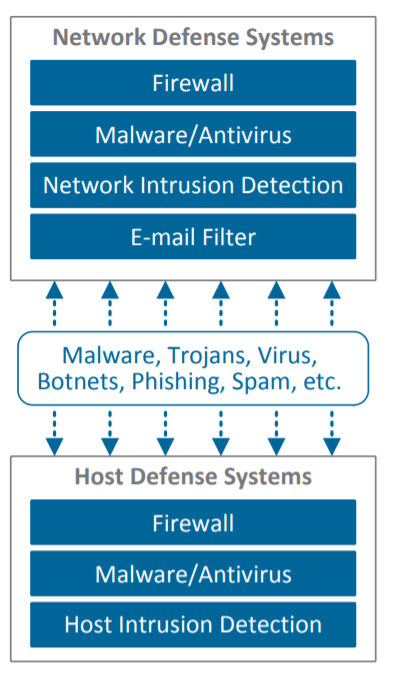
\includegraphics[width=0.7\linewidth]{secdnlp1}      
     \end{center}
    \end{column}
    \begin{column}{0.45\linewidth}
		\begin{itemize}
		\item  Cyber-threats are met by network defense systems including firewall, malware
software, and intrusion detection systems. 
\item Email protection typically occurs on network servers.
		\end{itemize}
		

    \end{column}
  \end{columns}

  \tiny{(Ref: Deep Learning for Cyber Security Usecases -  Technica Innovation
Platform White Paper)}
\end{frame}

%%%%%%%%%%%%%%%%%%%%%%%%%%%%%%%%%%%%%%%%%%%%%%%%%%%%%%%%%%
\begin{frame}[fragile]\frametitle{Top Attacks}
From a survey conducted by the ``Information 
Systems Audit and Control Association, Inc.'' (ISACA) 
and `RSA Security'', the Daily \% attacks are:
	
	
		\begin{itemize}
		\item Phishing 29.67
		\item Malicious Code 16.36
		\item Physical Loss 1.42
		\item Hacking 11.06
		\end{itemize}


\end{frame}


% %%%%%%%%%%%%%%%%%%%%%%%%%%%%%%%%%%%%%%%%%%%%%%%%%%%%%%%%%%
% \begin{frame}[fragile]\frametitle{Domains}
% Survey respondents found following areas topics of interest wrt Cyber Security
% \begin{itemize}
% \item  Internet of Things (IoT)
% \item  Industrial Control Systems and the Industrial IoT
% \item  Encryption
% \item  AI and Machine Learning 
% \end{itemize}

% \end{frame}

%%%%%%%%%%%%%%%%%%%%%%%%%%%%%%%%%%%%%%%%%%%%%%%%%%%%%%%%%%
\begin{frame}[fragile]\frametitle{Phishing Detection}
\begin{itemize}
\item  Attackers carefully craft emails mimicking 
valid communications from a company or individual familiar to employees.
\item  To trick recipients into providing access to their accounts.
\item One compromised account can provide attackers with credentials to
infiltrate a network, escalate privileges, gain access to core enterprise resource,
and steal sensitive data
\item ML/DL: Trained by a large number of analyzed emails, real-time alerts could be rendered
by the system to flag threats before they morph into data breaches.
\end{itemize}


\end{frame}

% %%%%%%%%%%%%%%%%%%%%%%%%%%%%%%%%%%%%%%%%%%%%%%%%%%%%%%%%%%
% \begin{frame}[fragile]\frametitle{Malware, Zero Day}
% \begin{itemize}
% \item  Deep learning-based malware detection algorithms
% can more adeptly detect malware—even zero day attacks, by  classifying malicious code without an expert creating rules
% that explicitly define malicious code. 
% \item Training the malware detection neural network would involve analysis of many
% millions of malicious and legitimate files for accurate classification.
% \item Once the neural network was trained, a small agent would be deployed on
% endpoint devices. 
% \end{itemize}
% \end{frame}

% %%%%%%%%%%%%%%%%%%%%%%%%%%%%%%%%%%%%%%%%%%%%%%%%%%%%%%%%%%
% \begin{frame}[fragile]\frametitle{Insider Threats}
% \begin{itemize}
% \item  A rapid change in the usage and communication pattern of an individual can be a
% sign of an upcoming insider attack

% \item Employees' demographic data and/or behavioral patterns could also extracted
% from access logs, traffic, etc. to indicate fraudulent activity. 
% \end{itemize}
% \end{frame}



% %%%%%%%%%%%%%%%%%%%%%%%%%%%%%%%%%%%%%%%%%%%%%%%%%%%%%%%%%%
% \begin{frame}[fragile]\frametitle{ Network Anomaly Detection}
% \begin{itemize}
% \item  Current Intrusion Detection Systems (IDS) and firewalls work through a
% combination of misuse detection techniques or anomaly detection techniques. 
% \item Deep learning based
% systems can be created to make better predictions of intrusions. 
% \item Smart filtering
% could adaptively point nefarious actors to honeypots for further analysis.
% \end{itemize}
% \end{frame}

% %%%%%%%%%%%%%%%%%%%%%%%%%%%%%%%%%%%%%%%%%%%%%%%%%%%%%%%%%%
% \begin{frame}[fragile]\frametitle{ Phishing Sites Detection}
% \begin{itemize}
% \item  OpenDNS’ Security Labs have developed NLPRank,to detect phishing sites set up by APT (Advanced Persistent Threat) actors
% \item Mails came from malicious domains whose names were constructed by using names of tech companies (Microsoft, Adobe, Firefox, Facebook, Java, GMail etc.)
% \item Used words like “login,” “update,” “security center,” “register,” “billing,” and so on. 
% \item It already has corpus of large number of DNS names, plus it uses certain WHOIS data patterns (for example, if the domain was registered just days or hours before), analyzes the sites’ HTML tags and ASN data.
% \end{itemize}

% \tiny{(Ref: NLPRank: An innovative tool for blocking APT malicious domains - Zeljka Zorz)}
% \end{frame}


%%%%%%%%%%%%%%%%%%%%%%%%%%%%%%%%%%%%%%%%%%%%%%%%%%%%%%%%%%
\begin{frame}[fragile]\frametitle{ Phishing Emails Detection}
\begin{itemize}
\item  Common phishing emails pretending to be notifications from trusted organizations (banks, Amazon, Netflix, etc.) that require the recipient to log into their account to fix the issue. 
\item By setting up a website that mimics the legitimate site, attackers can collect login credentials and other personal information.
\end{itemize}

\tiny{(Ref: How Companies Are Detecting Spear Phishing Attacks Using Machine Learning BY ANDREW GOLDBERG)}
\end{frame}

% %%%%%%%%%%%%%%%%%%%%%%%%%%%%%%%%%%%%%%%%%%%%%%%%%%%%%%%%%%
% \begin{frame}[fragile]\frametitle{User communication profiling}
% \begin{itemize}
% \item  Everyone has their own unique style of writing emails. 
% \item  Generally applicable: a few CEOs include emoticons or text message abbreviations in their official communications
% \item More specific: someone may have a favorite phrase that they use frequently
% \item These idiosyncrasies can be used to help detect and protect against phishing emails.
% \item NLP (Natural Language Processing) can be used effectively for this purpose.
% \end{itemize}

% \tiny{(Ref: How Companies Are Detecting Spear Phishing Attacks Using Machine Learning BY ANDREW GOLDBERG)}
% \end{frame}

%%%%%%%%%%%%%%%%%%%%%%%%%%%%%%%%%%%%%%%%%%%%%%%%%%%%%%%%%%
\begin{frame}[fragile]\frametitle{NLP}
\begin{itemize}
\item  Using NLP techniques, it is possible to analyze written text and extract identifying features from it. 
\item For example, the use of a dangling preposition (like the "for" in "What do you want that for?") is more common in some areas (and the people who grew up in those areas) than others. 
\item Also, people have different vocabularies, and a simple statistical analysis of word and phrase choice and preferred sentence structure and complexity can help to differentiate the writing of different people.
\end{itemize}

\tiny{(Ref: How Companies Are Detecting Spear Phishing Attacks Using Machine Learning BY ANDREW GOLDBERG)}

Such analysis is very challenging and is the Hall mark of ``Artificial Intelligence''. 

\textbf{NLP (using Deep Learning) is the way forward!!!}


\end{frame}
